\documentclass[10pt]{article}
\usepackage[margin=.72in]{geometry}
\usepackage[T1]{fontenc}
\usepackage{lmodern,microtype,booktabs,graphicx,xcolor,hyperref,placeins}
\definecolor{navy}{HTML}{16324F}\definecolor{teal}{HTML}{087E8B}
\hypersetup{colorlinks=true,linkcolor=navy,urlcolor=teal}
\title{\textcolor{navy}{Is the Local-Adaptation Gain a Capacity Effect?}\\[3pt]
\large A matched-function-class control across tasks, mechanisms and delays}
\author{23I-2581 and 23I-2604\\Data Analysis and Visualization --- Phase 3 research addendum}
\date{18 November 2026}
\begin{document}\maketitle
\begin{abstract}
Earlier matched-update experiments found that cluster-local refitting can outperform a single global logistic refit, but the local arm has greater representational capacity. We add a pooled cluster-interaction logistic control with the same 27 intercept/slope parameters as three separate cluster experts. All arms begin from the identical historical global model. Across 30 paired seeds, three task families, four mechanisms and delays 0/5/20, the interaction and local arms have nearly identical mean results. This supports a capacity-based explanation for much of the local--global gap in this design; it does not show that IDM-Viz's monitoring or triggering policy caused that gain.
\end{abstract}
\section{Question and design}
The primary contrast is a frozen classifier, one global logistic refit, three frozen-cluster local logistic experts, and a single pooled logistic model whose feature vector is block-coded by the same three frozen clusters. The latter has $3(8+1)=27$ parameters: one intercept and eight feature coefficients per cluster. The local arm fits the same function class as three separate models. Both adaptive arms start from the exact same global historical model and update at clocks 25, 49, 73 and 89 using the same latest released feedback-row IDs. Every arm is evaluated on the same streams; a row label is eligible only when its release precedes the prediction batch. Each adaptive opportunity is limited to 2,000 released rows and cumulative repeated row-use is capped at 8,000.

We evaluate 30 reserved seeds over linear, XOR and five-region synthetic tasks; stationary, gradual predictive, recurrent reversal and out-of-support mechanisms; and delays of 0, 5 and 20 batches. The seed is the resampling unit. Figure intervals use a paired seed-level max-$t$ bootstrap simultaneous across the 36 local--global contrasts; pointwise intervals remain in the CSV for reference. This is a sensitivity analysis, not universal inference.
\section{Results}
\begin{figure}[ht]
\centering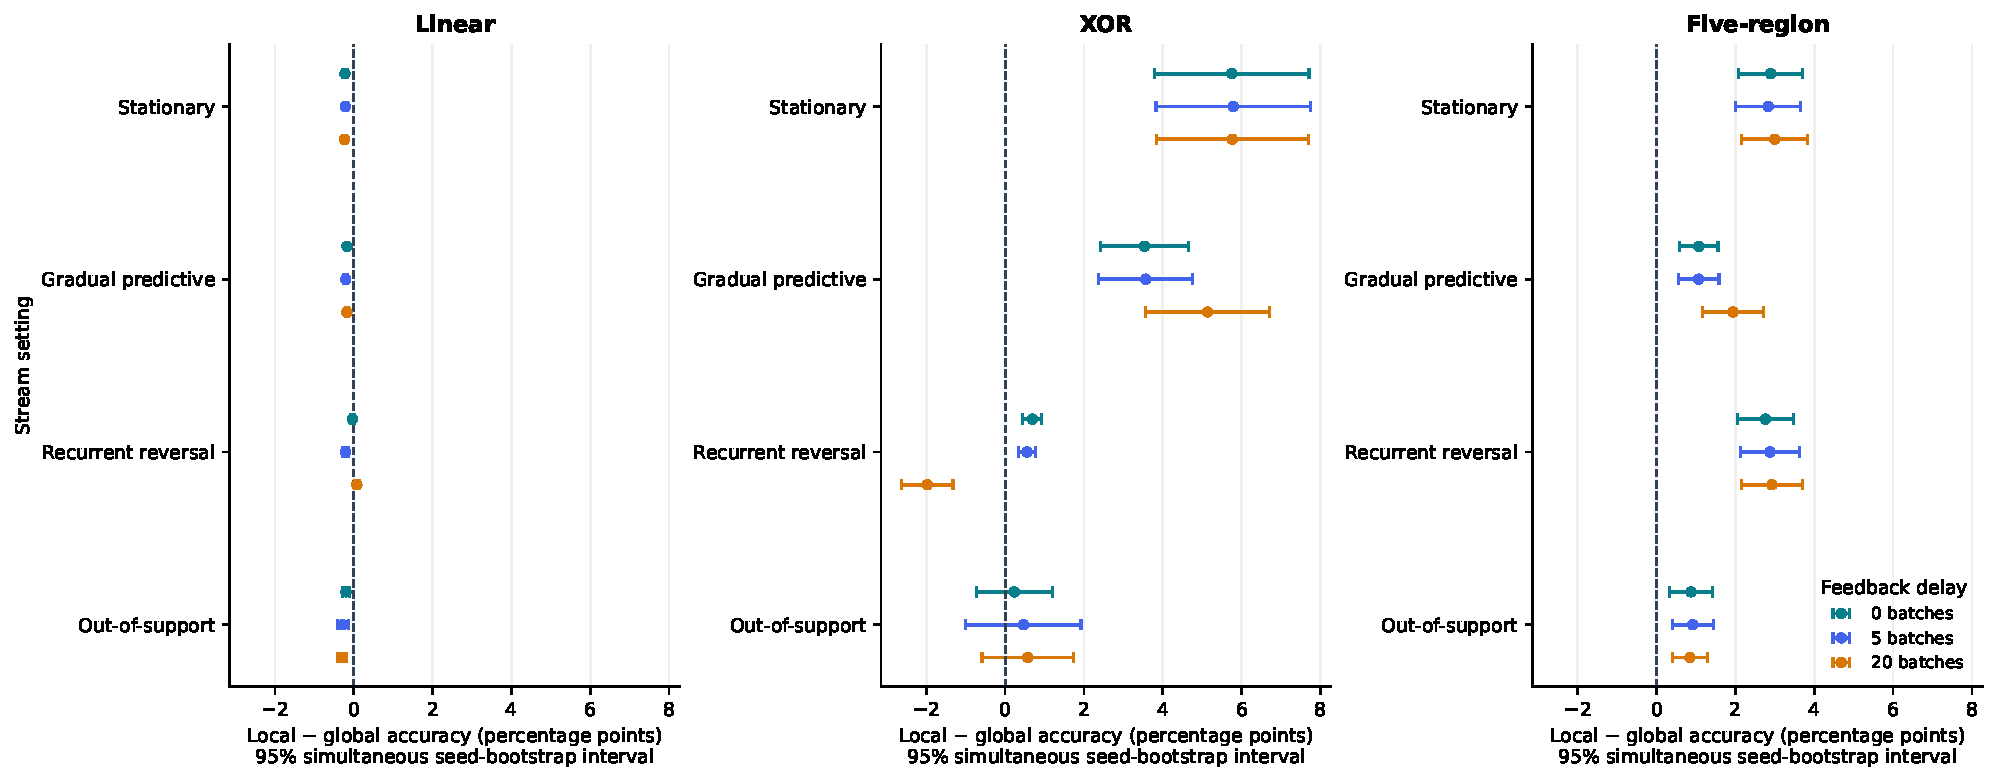
\includegraphics[width=\linewidth]{capacity_control_effects.pdf}
\caption{Local minus global accuracy, percentage points, paired over 30 seeds. Bars are 95\% max-$t$ bootstrap intervals simultaneous across all 36 task/mechanism/delay contrasts.}
\end{figure}
\begin{table}[ht]
\centering\small\begin{tabular}{@{}lrrrr@{}}\toprule
Task (nonstationary mechanisms) & Frozen & Global & Local & Interaction\\\midrule
Linear & 0.688 & 0.679 & 0.677 & 0.677 \\
XOR & 0.629 & 0.659 & 0.673 & 0.673 \\
Five-region & 0.542 & 0.580 & 0.597 & 0.597 \\\bottomrule\end{tabular}
\caption{Accuracy averaged across the three delays, four nonstationary mechanisms and 30 seeds. These averages summarize this designed simulation matrix.}\end{table}
\FloatBarrier
\section{Interpretation}
Only 32 of the 36 simultaneous intervals exclude zero. Original pointwise bootstrap intervals are retained alongside the simultaneous limits in the machine-readable effects table.
The interaction control closely reproduces the local arm's average accuracy in each task family: 0.5865 versus 0.5865 in five-region, 0.6885 versus 0.6886 in linear, and 0.6632 versus 0.6632 in XOR. In contrast, global-refit averages are 0.5665, 0.6904 and 0.6382. Thus the local--global difference is concentrated in the cluster-conditional function class, rather than evidence that separately fitting local experts or a local trigger is inherently better. The interaction model exceeds the global model in nonlinear/region-dependent tasks and underperforms it slightly in the linear task. This is consistent with a representation-by-task interaction.

The stationary condition is an important negative control: the same cluster-conditional function class also improves the five-region and XOR accuracy there. Consequently, the observed gap cannot be attributed solely to responding to drift. Recurrent reversal and delay effects are heterogeneous; aggregation over tasks or mechanisms would conceal failures. Local and interaction estimates are near-equivalent, but they are not a comparison of equal computational cost: the receipt records total fit wall time of about 95.6 seconds for local versus 204.4 seconds for interaction across this run, and wall time is hardware/software dependent.
\section{Validity checks and limitations}
The completed run contains 4,320 seed/task/mechanism/delay/method cells, 414,720 persisted batch forecasts and 21,600 fit-audit rows. The receipt records matched feedback hashes, four successful update opportunities, the 8,000 repeated-use cap, and source/config/output checksums. Across the run, 549 cluster-level fits fell back to the historical global model; these are repeated across seed/task/mechanism/delay/update combinations, and fallback frequency and effective row use are logged. The pooled interaction fitting objective and separate local fits are not guaranteed to converge identically in finite numerical optimization, despite their equivalent block function class. The simulation uses one classifier family and one fixed three-cluster partition. It does not demonstrate natural-stream transfer, causal attribution, analyst benefit, detector validity, or a deployment-ready adaptive policy. Threshold selection and trigger value are not tested by this fixed-clock comparison.
\section{Conclusion}
This control strengthens the interpretation of the earlier adaptation result: gains attributed to local adaptation are substantially explained by a cluster-conditional model class. IDM-Viz should describe this as evidence that regional representation can matter in the tested synthetic tasks, not evidence that the full monitoring framework yields a general accuracy improvement. The result motivates future matched-function-class and matched-compute comparisons on independent real streams.
\end{document}
